\documentclass[tikz]{standalone}
\usepackage{tkz-euclide}
\begin{document}
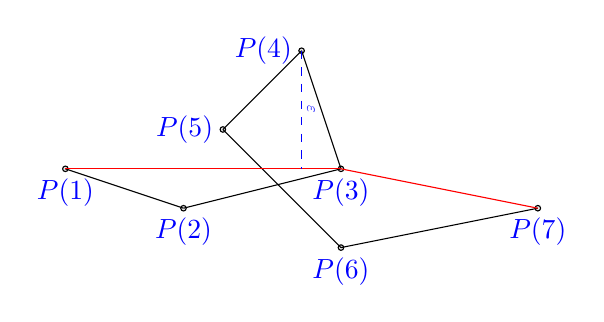
\begin{tikzpicture}[scale=0.5]
	\tkzInit[xmax=13,ymax=8,xmin=-1,ymin=-1]
	
	\tkzDefPoint(0,2){1}
	\tkzDefPoint(3,1){2}
	\tkzDefPoint(7,2){3}
	\tkzDefPoint(6,5){4}
	\tkzDefPoint(4,3){5}
	\tkzDefPoint(7,0){6}
	\tkzDefPoint(12,1){7}

	\tkzDefPoint(6,2){temp}

	\tkzDrawPoints(1,2,3,4,5,6,7)

	\path[-] (1) edge (2);
	\path[-] (2) edge (3);
	\path[-] (3) edge (4);
	\path[-] (4) edge (5);
	\path[-] (5) edge (6);
	\path[-] (6) edge (7);

	\tkzLabelPoint[color=blue](1){$P(1)$}
	\tkzLabelPoint[color=blue](2){$P(2)$}
	\tkzLabelPoint[color=blue](3){$P(3)$}
	\tkzLabelPoint[color=blue, left](4){$P(4)$}
	\tkzLabelPoint[color=blue, left](5){$P(5)$}
	\tkzLabelPoint[color=blue](6){$P(6)$}
	\tkzLabelPoint[color=blue](7){$P(7)$}
	\path[-,color=red] (1) edge (3);
	\path[-,color=red] (3) edge (7);
	\path[dashed,color=blue] (4) edge node[above,sloped,scale=0.6]{$\varepsilon$}(temp);
\end{tikzpicture}
\end{document}
